上の設計を通して、以下のようなコードによってpprofを起動することができます:


\begin{lstlisting}[numbers=none]
beego.PprofOn = true
\end{lstlisting}

次に、ブラウザで以下のURLを開くと以下のようなインターフェースが現れます: 

\begin{figure}[H]
   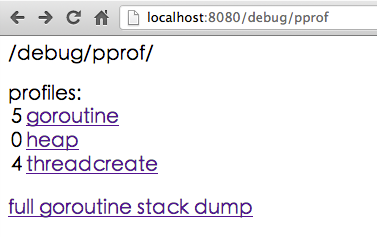
\includegraphics[width=7cm]{14.6.pprof.png}
   \label{図14.7}
   \caption{システムの現在のgoroutine、heap、threadの情報}
\end{figure}

goroutineをクリックすると詳細な情報を得ることができます:


\begin{figure}[H]
   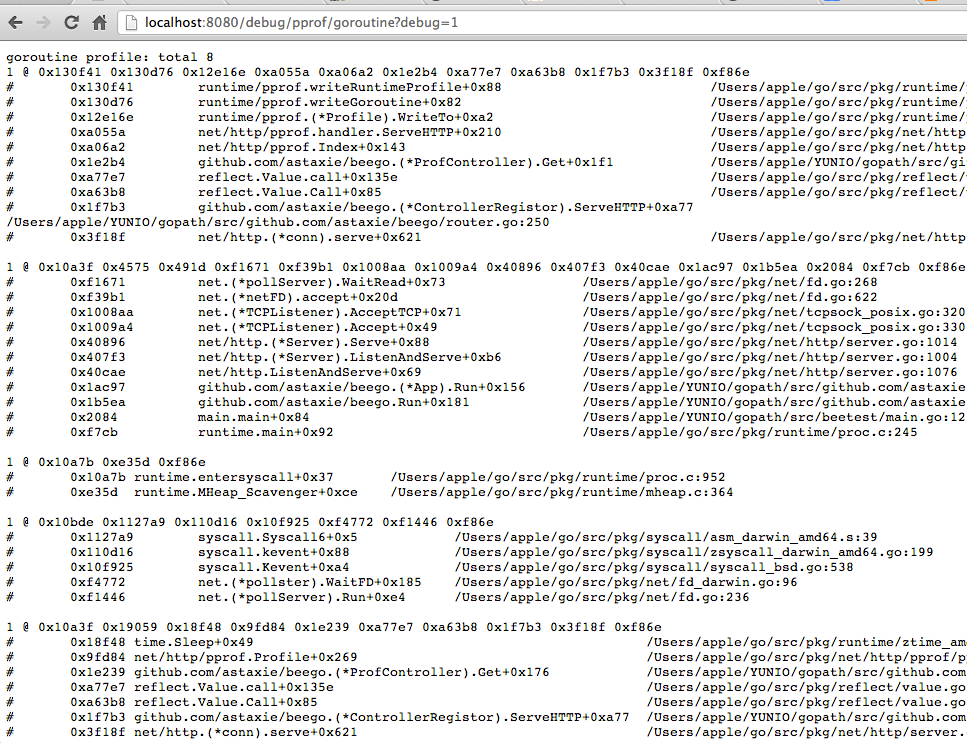
\includegraphics[width=14cm]{14.6.pprof2.png}
   \label{図14.8}
   \caption{現在のgoroutineの詳細情報を表示}
\end{figure}

コマンドラインから更に多くの詳細な情報を得ることもできます

\begin{lstlisting}[numbers=none]
go tool pprof http://localhost:8080/debug/pprof/profile
\end{lstlisting}

この時、プログラムは30秒のprofile収集時間に入ります。この時間内に必死にブラウザ上のページをリロードし、なるべくcpuを専有させてデータを生成します。



\begin{lstlisting}[numbers=none]
(pprof) top10

Total: 3 samples

   1 33.3% 33.3% 1 33.3% MHeap_AllocLocked

   1 33.3% 66.7% 1 33.3% os/exec.(*Cmd).closeDescriptors

   1 33.3% 100.0% 1 33.3% runtime.sigprocmask

   0 0.0% 100.0% 1 33.3% MCentral_Grow

   0 0.0% 100.0% 2 66.7% main.Compile

   0 0.0% 100.0% 2 66.7% main.compile

   0 0.0% 100.0% 2 66.7% main.run

   0 0.0% 100.0% 1 33.3% makeslice1

   0 0.0% 100.0% 2 66.7% net/http.(*ServeMux).ServeHTTP

   0 0.0% 100.0% 2 66.7% net/http.(*conn).serve    

(pprof)web
\end{lstlisting}


\begin{figure}[H]
   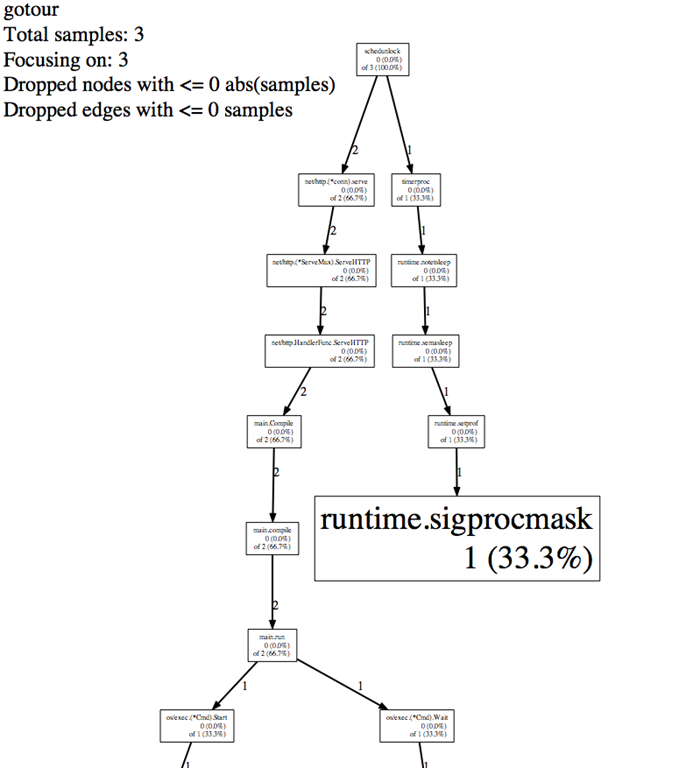
\includegraphics[width=14cm]{14.6.pprof3.png}
   \label{図14.9}
   \caption{デモの実行プロセス情報}
\end{figure}

